\documentclass[border=3pt]{standalone}
% Shared preamble for standalone figures (same fonts/colours as the paper).
\usepackage[T1]{fontenc}
\usepackage{lmodern}
\usepackage{amsmath,amssymb}
\usepackage[dvipsnames,svgnames]{xcolor}
\usepackage{tikz}
\usetikzlibrary{arrows.meta,positioning,calc,shapes.geometric,decorations.pathreplacing,shadings}
\usepackage{pgfplots}
\pgfplotsset{compat=1.18}
\usepgfplotslibrary{fillbetween}
\definecolor{pgrey}{HTML}{EEEEEE}
\definecolor{ppink}{HTML}{F8D7DA}
\definecolor{ppeach}{HTML}{FDE5C8}
\definecolor{porange}{HTML}{FBC78D}
\definecolor{pgreen}{HTML}{D4F7D4}
\definecolor{ppurple}{HTML}{EFE3F7}
\definecolor{pblue}{HTML}{DCE8F7}
\definecolor{dgreen}{HTML}{2E8B2E}
\definecolor{dpink}{HTML}{C2185B}
\definecolor{dorange}{HTML}{E07B00}
\definecolor{dblue}{HTML}{1F4E9E}
\definecolor{dpurple}{HTML}{7B3FA0}
\definecolor{gold}{HTML}{E0A800}
\tikzset{
  blk/.style={draw=black!70,rounded corners=2pt,minimum height=0.8cm,minimum width=1.9cm,
              align=center,font=\sffamily\footnotesize,inner sep=3pt},
  arr/.style={-{Stealth[length=2.2mm]},thick,black!75},
  darr/.style={-{Stealth[length=2mm]},dashed,thick},
  lbl/.style={font=\itshape\scriptsize},
}

\begin{document}
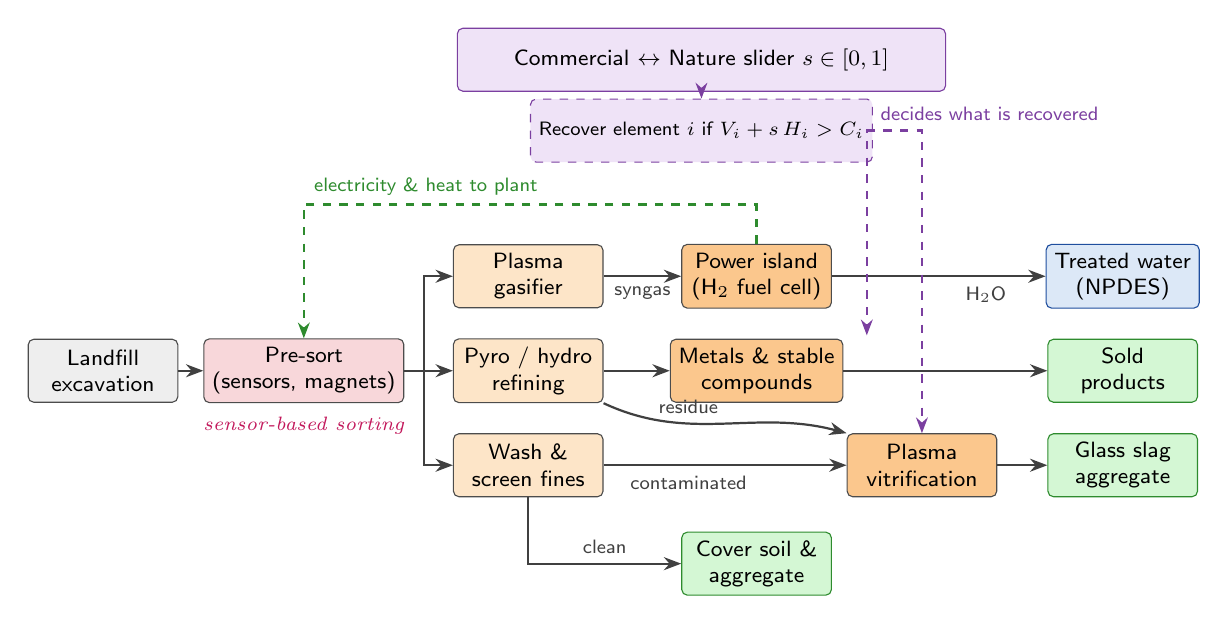
\begin{tikzpicture}
% control layer
\node[blk,fill=ppurple,draw=dpurple,minimum width=6.2cm] (slider) at (7.6,3.95)
  {Commercial $\leftrightarrow$ Nature slider $s\in[0,1]$};
\node[blk,fill=ppurple,draw=dpurple,dashed,minimum width=3.4cm,font=\sffamily\scriptsize] (crit) at (7.6,3.05)
  {Recover element $i$ if $V_i + s\,H_i > C_i$};
\draw[darr,dpurple] (slider) -- (crit);
% main line
\node[blk,fill=pgrey] (fill) at (0,0) {Landfill\\excavation};
\node[blk,fill=ppink] (sort) at (2.55,0) {Pre-sort\\(sensors, magnets)};
\node[lbl,text=dpink,below=0.05cm of sort] {sensor-based sorting};
\node[blk,fill=ppeach] (gas)  at (5.4,1.2)  {Plasma\\gasifier};
\node[blk,fill=ppeach] (ref)  at (5.4,0)    {Pyro / hydro\\refining};
\node[blk,fill=ppeach] (wash) at (5.4,-1.2) {Wash \&\\screen fines};
\node[blk,fill=porange] (power) at (8.3,1.2) {Power island\\(H$_2$ fuel cell)};
\node[blk,fill=porange] (stab) at (8.3,0)  {Metals \& stable\\compounds};
\node[blk,fill=porange] (vit)  at (10.4,-1.2) {Plasma\\vitrification};
\node[blk,fill=pgreen,draw=dgreen] (metals) at (12.95,0) {Sold\\products};
\node[blk,fill=pgreen,draw=dgreen] (soil) at (8.3,-2.45) {Cover soil \&\\aggregate};
\node[blk,fill=pgreen,draw=dgreen] (slag) at (12.95,-1.2) {Glass slag\\aggregate};
\node[blk,fill=pblue,draw=dblue] (water) at (12.95,1.2) {Treated water\\(NPDES)};
% flows
\draw[arr] (fill) -- (sort);
\draw[arr] (sort.east) -- ++(0.25,0) |- (gas.west);
\draw[arr] (sort) -- (ref);
\draw[arr] (sort.east) -- ++(0.25,0) |- (wash.west);
\draw[arr] (gas) -- node[below,font=\sffamily\scriptsize]{syngas} (power);
\draw[arr] (ref) -- (stab);
\draw[arr] (stab) -- (metals);
\draw[arr] (power) -- node[pos=0.72,below,font=\sffamily\scriptsize]{H$_2$O} (water);
\draw[arr] (wash) |- node[pos=0.75,above,font=\sffamily\scriptsize]{clean} (soil);
\draw[arr] (wash) -- node[pos=0.35,below,font=\sffamily\scriptsize]{contaminated} (vit);
\draw[arr] (ref.south east) to[out=-25,in=165] node[pos=0.35,above,font=\sffamily\scriptsize]{residue} (vit.north west);
\draw[arr] (vit) -- (slag);
% energy loop
\draw[darr,dgreen] (power.north) -- ++(0,0.5) -| (sort.north);
\node[font=\sffamily\scriptsize,text=dgreen,above] at (4.1,2.1) {electricity \& heat to plant};
% control arrows
\draw[darr,dpurple] (crit.east) -- (9.7,3.05) -- (9.7,0.45);
\draw[darr,dpurple] (9.7,3.05) -| (vit.north);
\node[font=\sffamily\scriptsize,text=dpurple,anchor=south west] at (9.75,3.05) {decides what is recovered};
\end{tikzpicture}
\end{document}
